%%%%%%%%%%%%%%%%%%%%%%%%%%%%%%%%%%%%%%%%%
% Professional Newsletter Template
% LaTeX Template
% Version 1.0 (09/03/14)
%
% Created by:
% Bob Kerstetter (https://www.tug.org/texshowcase/) and extensively modified by:
% Vel (vel@latextemplates.com)
% 
% This template has been downloaded from:
% http://www.LaTeXTemplates.com
%
% License:
% CC BY-NC-SA 3.0 (http://creativecommons.org/licenses/by-nc-sa/3.0/)
%
%%%%%%%%%%%%%%%%%%%%%%%%%%%%%%%%%%%%%%%%%

\documentclass[10pt]{article} % The default font size is 10pt; 11pt and 12pt are alternatives

%%%%%%%%%%%%%%%%%%%%%%%%%%%%%%%%%%%%%%%%%
% Professional Newsletter Template
% Structural Definitions File
% Version 1.0 (09/03/14)
%
% Created by:
% Vel (vel@latextemplates.com)
% 
% This file has been downloaded from:
% http://www.LaTeXTemplates.com
%
% License:
% CC BY-NC-SA 3.0 (http://creativecommons.org/licenses/by-nc-sa/3.0/)
%
%%%%%%%%%%%%%%%%%%%%%%%%%%%%%%%%%%%%%%%%%

%----------------------------------------------------------------------------------------
%	REQUIRED PACKAGES
%----------------------------------------------------------------------------------------

\usepackage{graphicx} % Required for including images
\usepackage{microtype} % Improved typography
\usepackage{multicol} % Used for the two-column layout of the document
\usepackage{booktabs} % Required for nice horizontal rules in tables
\usepackage{wrapfig} % Required for in-line images
\usepackage{float} % Required for forcing figures not to float with the [H] parameter

%------------------------------------------------
% Fonts

\usepackage{charter} % Use the Charter font as the main document font
\usepackage{courier} % Use the Courier font for \texttt (monospaced) only
\usepackage[T1]{fontenc} % Use T1 font encoding

%------------------------------------------------
% List Separation

\usepackage{enumitem} % Required to customize the list environments
\setlist{noitemsep,nolistsep} % Remove spacing before, after and within lists for a compact look

%------------------------------------------------
% Figure and Table Caption Styles

\usepackage{caption} % Required for changing caption styles
\captionsetup[table]{labelfont={bf,sf},labelsep=period,justification=justified} % Specify the table caption style
\captionsetup[figure]{labelfont={sf,bf},labelsep=period,justification=justified, font=small} % Specify the figure caption style
\setlength{\abovecaptionskip}{10pt} % Whitespace above captions

%------------------------------------------------
% Spacing Between Paragraphs

\makeatletter
\usepackage{parskip}
\setlength{\parskip}{6pt}
\newcommand{\@minipagerestore}{\setlength{\parskip}{6pt}}
\makeatother

%----------------------------------------------------------------------------------------
%	PAGE MARGINS AND SPACINGS
%----------------------------------------------------------------------------------------

\textwidth = 7 in % Text width
\textheight = 10 in % Text height
\oddsidemargin = -18pt % Left side margin on odd pages
\evensidemargin = -18pt % Left side margin on even pages
\topmargin = -36pt % Top margin
\headheight = 0pt % Remove the header by setting its space to 0
\headsep = 0pt % Remove the space between the header and top of the page
\parskip = 4pt % Space between paragraph
\parindent = 0.0in % Paragraph indentation
\pagestyle{empty} % Disable page numbering

%----------------------------------------------------------------------------------------
%	COLORS
%----------------------------------------------------------------------------------------

\usepackage[dvipsnames,svgnames]{xcolor} % Required to specify custom colors

\definecolor{altncolor}{rgb}{.8,0,0} % Dark red
%\definecolor{altncolor}{rgb}{.2,.4,.8} % Dark blue
%\definecolor{altncolor}{rgb}{.84,.16,.16} % Red

\usepackage[colorlinks=true, linkcolor=altncolor, anchorcolor=altncolor, citecolor=altncolor, filecolor=altncolor, menucolor=altncolor, urlcolor=altncolor]{hyperref} % Use the color defined above for all links

%----------------------------------------------------------------------------------------
%	BOX STYLES
%----------------------------------------------------------------------------------------

\usepackage[framemethod=TikZ]{mdframed}% Required for creating boxes
\mdfdefinestyle{sidebar}{
    linecolor=black, % Outer line color
    outerlinewidth=0.5pt, % Outer line width
    roundcorner=0pt, % Amount of corner rounding
    innertopmargin=10pt, % Top margin
    innerbottommargin=10pt, % Bottom margin
    innerrightmargin=10pt, % Right margin
    innerleftmargin=10pt, % Left margin
    backgroundcolor=white, % Box background color
    frametitlebackgroundcolor=white, % Title background color
    frametitlerule=false, % Title rule - true or false
    frametitlerulecolor=white, % Title rule color
    frametitlerulewidth=0.5pt, % Title rule width
    frametitlefont=\Large, % Title heading font specification
    font=\small
}

\mdfdefinestyle{intextbox}{
    linecolor=black, % Outer line color
    outerlinewidth=0.5pt, % Outer line width
    roundcorner=10pt, % Amount of corner rounding
    innertopmargin=7pt, % Top margin
    innerbottommargin=7pt, % Bottom margin
    innerrightmargin=7pt, % Right margin
    innerleftmargin=7pt, % Left margin
    backgroundcolor=white, % Box background color
    frametitlebackgroundcolor=white, % Title background color
    frametitlerule=false, % Title rule - true or false
    frametitlerulecolor=white, % Title rule color
    frametitlerulewidth=0.5pt, % Title rule width
    frametitlefont=\Large % Title heading font specification
}

%----------------------------------------------------------------------------------------
%	HEADING STYLE
%----------------------------------------------------------------------------------------

\newcommand{\heading}[2]{ % Define the \heading command
\vspace{#2} % White space above the heading
{\begin{center}\Large\textbf{#1}\end{center}} % The heading style
\vspace{#2} % White space below the heading
}

\newcommand{\BackToContents}{\hyperlink{contents}{{\small Back to Contents}}} % Define a command for linking back to the contents of the newsletter % Include the document which specifies all packages and structural customizations for this template
\usepackage{soul}
\setuldepth{Berlin}
\usepackage{lettrine}
\usepackage{amsmath}
\usepackage{nicefrac}
\usepackage{booktabs}

\usepackage[usestackEOL]{stackengine}
%\usepackage{libertine}
\usepackage{fancyhdr}
% Turn on the style
\pagestyle{fancy}
% Clear the header and footer
\fancyhead{}
\fancyfoot{}
\renewcommand{\headrulewidth}{0pt}
% Set the right side of the footer to be the page number
\fancyfoot[r]{\thepage}
%\usepackage{showframe}


\setlength{\footskip}{1\baselineskip}

\begin{document}
	
	%----------------------------------------------------------------------------------------
	%	HEADER IMAGE
	%----------------------------------------------------------------------------------------
	
	%\begin{figure}[H]
	%\centering
\includegraphics[width=0.3\linewidth]{logo.png}
	%\end{figure}
	\centering \textsc{Poseidon: Open source Syringe Pump and Microscope}
	%----------------------------------------------------------------------------------------
	%	SIDEBAR - FIRST PAGE
	%----------------------------------------------------------------------------------------
	
	\begin{minipage}[t]{.30\linewidth} % Mini page taking up 30% of the actual page
		\begin{mdframed}[style=sidebar,frametitle={}] % Sidebar box
			
			%----------------------------------------------------------
			
			%\centerline {\rule{.75\linewidth}{.25pt}} % Horizontal line
			
			%-----------------------------------------------------------
			\textbf{\large Poseidon Quick Facts: }
			\centerline {\rule{.75\linewidth}{.25pt}} % Horizontal line			
			
			\begingroup
			\setstackgap{S}{2pt}
			\setlength{\tabcolsep}{3pt} % Default value: 6pt
			\renewcommand{\arraystretch}{1.5} % Default value: 1
			\begin{tabular}{@{}rl@{}}
				\textbf{\emph{Operation:}} & infuse \& withdraw \\
				\textbf{\emph{Total Cost:}} &\$500\\
				\textbf{\emph{Print time:}} & 20hr\\
				\textbf{\emph{Build time: }} & 20min\\
				\textbf{\emph{Syringe:}} & BD Plastic 1-60mL\\
				\textbf{\emph{Dist Units:}} & mm, mL, $\mu$L\\
				\textbf{\emph{Time units:}} & sec, min, hr\\
				\textbf{\emph{Pos. Tol:}} & $\pm$ 0.01 mm\\
				\textbf{\emph{Pos. Range:}} & 0-150mm\\
				\textbf{\emph{Speed Tol:}} & $\pm$ 0.01 mm/sec\\
				\textbf{\emph{Speed Range:}} & 0-$\infty$ mm/sec\\
				\textbf{\emph{Max Rate:}} & 0 mL/sec\\
				\textbf{\emph{Min Rate:}} & 0 mL/sec\\
				\textbf{\emph{Microscope:}} & 8x\\
			\end{tabular}
		\endgroup
			
			
			%\centerline {\rule{.75\linewidth}{.25pt}} % Horizontal line
			\vspace{6px}
			\textbf{\large Experiments are easy:} 
			\centerline {\rule{.75\linewidth}{.25pt}} % Horizontal line			
			
			Assuming components are connected and powered:
			
			\begin{enumerate}[leftmargin=*]
				\raggedright
				\item Launch the GUI by typing \texttt{python gui.pu}
				\item Load \texttt{testing.txt} by pressing \texttt{File -> Load Settings}
				\item Select the arduino port 
				\item Send the settings to the controller by pressing \texttt{send to controller}
				\item In the run tab, enable the pumps you want to run, and enter their displacements
				\item Press \texttt{run} on the run tab to start your experiment
				\item Pause or stop at any time by pressing \texttt{pause} or \texttt{stop}
			\end{enumerate}
			
			%-----------------------------------------------------------
			\vspace{10px}
			\textbf{\large Get started:}
			
			\centerline {\rule{.75\linewidth}{.25pt}} % Horizontal line			
			Check out the project page which has all of the files as well as detailed instructions on how to build (and hack) the system!
			\url{https://pachterlab.github.io/poseidon/}
			
			%-----------------------------------------------------------
			
%			\captionof*{table}{Table Caption}
%			\begin{tabular}{llr}
%				\toprule
%				\multicolumn{2}{c}{Name} \\
%				\cmidrule(r){1-2}
%				First & Last & Grade \\
%				\midrule
%				John & Doe & $7.5$ \\
%				Richard & Miles & $2$ \\
%				\bottomrule
%			\end{tabular}
			
			%-----------------------------------------------------------
			
		\end{mdframed}
	\end{minipage}\hfill % End the sidebar mini page 
	%
	%----------------------------------------------------------------------------------------
	%	MAIN BODY - FIRST PAGE
	%----------------------------------------------------------------------------------------
	%
	\begin{minipage}[t]{.66\linewidth} % Mini page taking up 66% of the actual page
		
		\hypertarget{firstnews}{\heading{On the development of the Poseidon System}{6pt}} % \hypertarget provides a label to reference using \hyperlink{label}{link text}
		\lettrine[lraise=0.1, nindent=0em, slope=-.5em]{T}{he} Poseidon system was developed as a highly modifiable and cheap alternative to currently available syringe pump and microscope systems. At 10x cheaper than current systems, and built using the \textit{Principles of Open Hardware Design}, Poseidon allows users to simply setup, modify, and run microfluidics experiments.
		
		\begin{center}
			\parbox[t]{.70\linewidth}{\emph{Principles of Open Hardware Design include: principle one, principle two, etc}}
		\end{center}
		
		\begin{wrapfigure}[9]{r}[0pt]{0pt} % In-line figure with text wrapping around it
			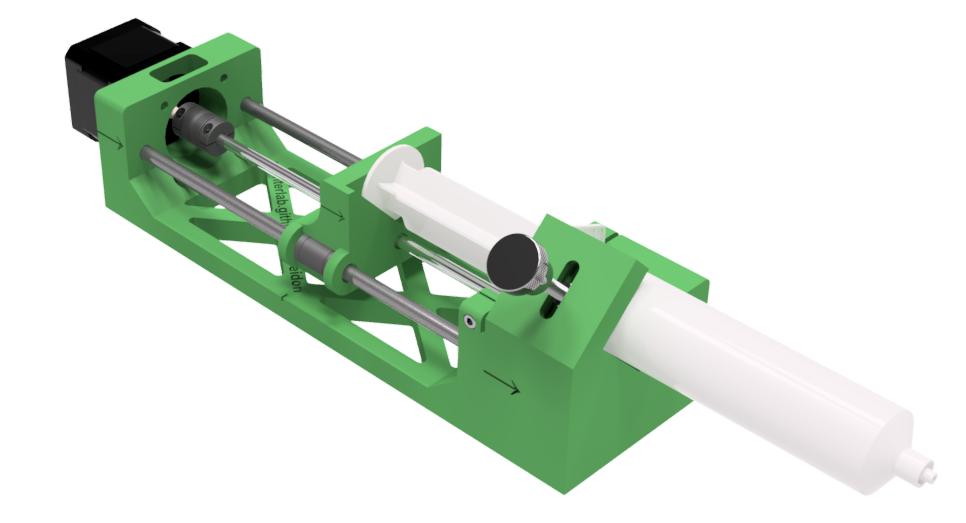
\includegraphics[width=0.4\textwidth]{img/pump-ortho.png}
		\end{wrapfigure}
		The Poseidon system includes a syringe pump and a microscope. These are two important components in any microfluidic experiment. Current pumping and vision systems include Harvard Apparatus, \textbf{insert other here}, Nikon desktop optical microscope, and \textbf{insert other here}. While these devices are used widly and have many unique features, they are expensive and many lack the ability to modify the operation of the device. 

		\begin{wrapfigure}[9]{l}[0pt]{0pt} % In-line figure with text wrapping around it
			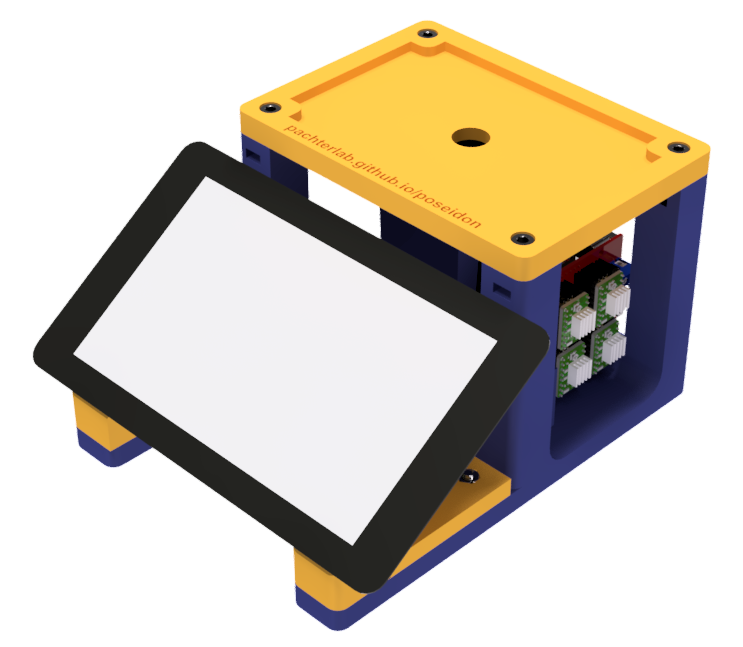
\includegraphics[width=0.33\textwidth]{img/cam-ortho.png}
		\end{wrapfigure}
		
		The Poseidon system was developed using entirely 3-D printed parts and components that are all easily sourced from Amazon. The syringe pump uses an arduino, compatible motor drivers, and Nema 17 stepper motor to drive a 0.8mm/step lead screw which in turn moves a sled that is mounted on linear bearings. The displacement of the sled moves the syringe forward or backward allowing the user to dispel or intake liquid. 
		
		The microscope was built using a raspberry
		 pi computer and USB microscope. The raspberry pi acts as a computer that controls the syringe pumps by sending move commands via the arduino microcontroller. 
		

	
		
		%-----------------------------------------------------------
		
		\hypertarget{secondnews}{\heading{On the hackability of the Poseidon System}{6pt}} % \hypertarget provides a label to reference using \hyperlink{label}{link text}
		
		Every user made component of the Poseidon system is hackable and modifiable. These include
		
		\begin{itemize}
			\item CAD (computer aided design) file of the 3-D printed components
			\item GUI (graphical user interface) and its layout
			\item Arduino sketch that runs the motors
			\item Controller code that connects commands from the GUI to the arduino
		\end{itemize}
		\begin{wrapfigure}{r}[0pt]{0pt} % In-line figure with text wrapping around it
			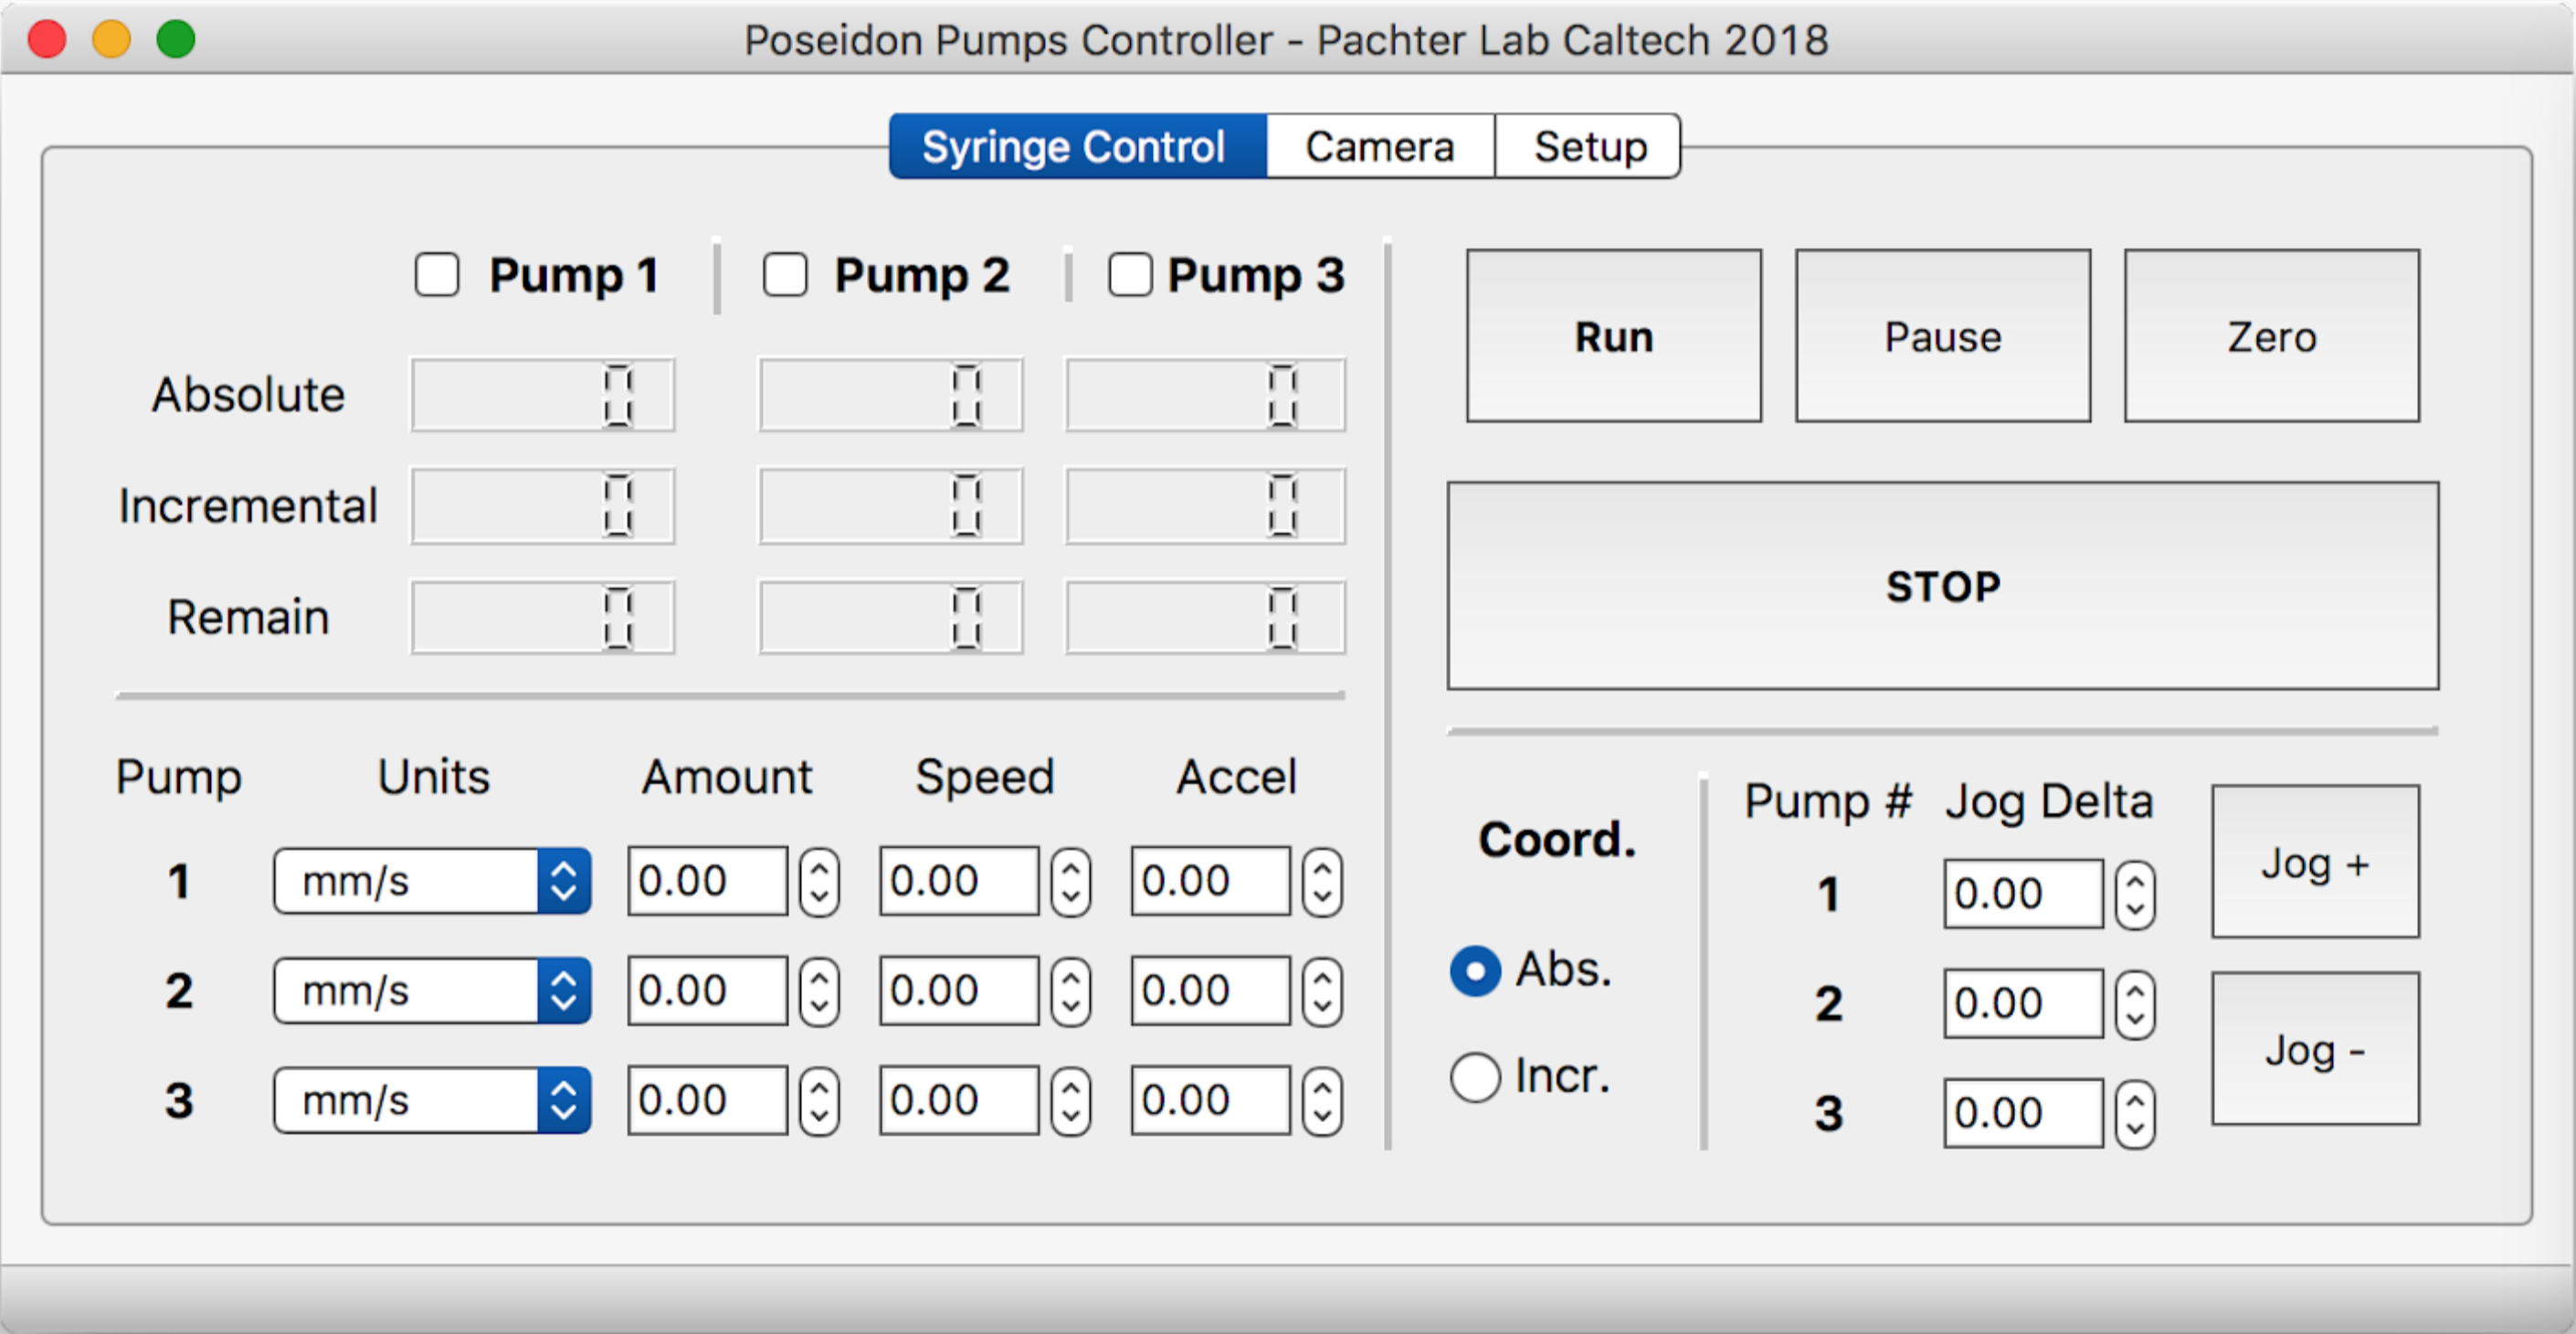
\includegraphics[width=0.5\textwidth]{img/gui-example.png}
		\end{wrapfigure}
		The 3-D printed components were designed using Fusion 360, a CAD software available free to students. To modify any 3-D printed part the user downloads Fusion 360, loads the files, and implements changes. These files can then be 3-D printed using available slicing software and printer. 
		
		The GUI was created using Qt designer, a drag and drop application for organizing buttons. The user can load the uiFileName.ui file and modify any buttons and inputs she desires. This new GUI can then be converted to a python file using \texttt{pyuic5 uiFileName.ui > uiFileName.py}.
		
	\end{minipage} % End the main body - first page mini page
	
	%----------------------------------------------------------------------------------------
	%	MAIN BODY - SECOND PAGE
	%----------------------------------------------------------------------------------------
	
	\begin{minipage}[t]{.66\linewidth} % Mini page taking up 66% of the actual page
		With the new ui python file, the user can configure which commands are sent to the controller when different elements of the GUI are activated (via a button press or checkbox toggle etc). These commands are sent to, and interpreted by the custom Arduino sketch.
		


		\begin{center}
	
			\begin{tabular}{@{}rl@{}}
				\multicolumn{2}{c}{ \texttt{<mode,setting,motor,value,dir,opt1,opt2,opt3>}} \\
				\toprule
				\cmidrule(r){1-2}
				Variable & Argument (sent as a string)\\
				\midrule
				mode & ["RUN", "SETTING", "JOG", "STOP"]\\
				setting & ["ALL"", "FEW", "ONE", "ACCEL", "SPEED", "DELTA"]\\
				motorID & [1, 2, 3, 12, 23, 13, 123] \\
				value & any positive floating number\\
				direction & ['F', 'B']\\
				opt1 & any floating number\\
				opt2 & any floating number\\
				opt3 & any floating number\\
				\bottomrule
			\end{tabular}
		\end{center}

		
		The Arduino interprets the custom commands that are sent by python, through the serial port (USB port), and executes the associated function on the board which in turn results in stepper motor movement. Certain commands require value inputs, such as distance to move, and in this case the Arduino is capable of grabbing those values from the python command and executing a local function with that value. The user can take advantage of this protocol by developing custom movement patterns using the Arduino functions. 
		
		
		
		
		
		\hypertarget{thirdnews}{\heading{On the licensing of the Poseidon System}{6pt}} % \hypertarget provides a label to reference using \hyperlink{label}{link text}
		
		\begin{multicols}{2} % Two-column layout
			This is still TBD but Eduardo is adamant about a certain license.
		\end{multicols}
		
		
		%----------------------------------------------------------------------------------------
		%	IN-TEXT BOX
		%----------------------------------------------------------------------------------------
		
%		\begin{mdframed}[style=intextbox,frametitle={}] % Sidebar box
%			
%			\hypertarget{descriptivebox}{\heading{Descriptive Box}{0pt}} % \hypertarget provides a label to reference using \hyperlink{label}{link text}
%			
%			Nam in turpis scelerisque libero luctus tincidunt sed faucibus lorem ac nisi rhoncus hendrerit. Praesent semper dui non justo rhoncus consequat. Mauris egestas tempus ligula:
%			\begin{enumerate}
%				\item Quisque mi metu.      
%				\item Sem iaculis molestie vulputate.
%				\item Suscipit accumsan dui metus sed.
%				\item Molestie sed ullamcorper quis, venenatis nec lorem.
%				\item Nec pulvinar \textsl{Rutrum Cursus / Ante\dots} command.      
%				\item Donec sit amet sem ligula,  \textsl{non} posuere neque. 
%				\item In hac habitasse nibh ultricies pellentesque elit risus sollicitudin velit.
%				\item Aliquam nec metus sed.
%			\end{enumerate}
%			
%			\BackToContents % Link back to the contents of the newsletter
%			
%		\end{mdframed}
		
		%----------------------------------------------------------------------------------------
		%	QUOTATION
		%----------------------------------------------------------------------------------------
		\centerline {\rule{.75\linewidth}{.25pt}} % Horizontal line	
		\hypertarget{quotation}{{\textbf{\large User Quotes}}} % \hypertarget provides a label to reference using \hyperlink{label}{link text}
		
		\begin{quote}
			\raggedright \textsl{I loved how easy the system was to setup!} \\ \raggedleft--- \textrm{L. Pachter (P.I.)}
		\end{quote}
	
		\begin{quote}
			\raggedright \textsl{Screw big corporations! I want to start my own big corporation using these pumps for profit. MWUAHAHA} \\ \raggedleft--- \textrm{E. D. V. Beltrame (Graduate Student)}
		\end{quote}
	
		\begin{quote}
			\raggedright \textsl{Finally a reliable, inexpensive, and hackable system that I can use for my Drop Seq experiments.} \\ \raggedleft--- \textrm{J. Gehring (Post Doc)}
		\end{quote}
		
		%----------------------------------------------------------------------------------------
		
	\end{minipage}\hfill % End of the main body - second page mini page
	\begin{minipage}[t]{.30\linewidth} % Mini page taking up 30% of the actual page
		
		%----------------------------------------------------------------------------------------
		%	SIDEBAR - SECOND PAGE
		%----------------------------------------------------------------------------------------
		
		\begin{mdframed}[style=sidebar,frametitle={}] % Sidebar box
			
			\heading{Tech Specs}{0pt}
			
			\centerline {\rule{.75\linewidth}{.25pt}} % Horizontal line	
			\begingroup
			\setstackgap{S}{3pt}
			\setlength{\tabcolsep}{3pt} % Default value: 6pt
			\renewcommand{\arraystretch}{1.5} % Default value: 1
			\begin{tabular}{@{}rl@{}}
				\textbf{\emph{Motor Type: }} & Nema 17\\
				\textbf{\emph{Motor Steps: }} & 200/rev\\
				\textbf{\emph{Screw pitch: }} & 0.8 mm/rev\\
				\textbf{\emph{Microstep: }} & $\nicefrac{1}{2} \,\, \nicefrac{1}{8}\,\, \nicefrac{1}{16}\,\, \nicefrac{1}{32}$\\
				\textbf{\emph{Dist per step: }} & 4 $\mu$m\\
				\textbf{\emph{Arduino Power: }} & 12V DC @ 2A\\
				\textbf{\emph{Raspi Power: }} & 5V DC @ 1A\\
			\end{tabular}
			\endgroup
			
		\end{mdframed}\hfill
		
		%----------------------------------------------------------------------------------------
		
		\centering
		\begin{minipage}[t]{.95\linewidth}
			\textbf{Contact Us:}\\
			Pachter Lab, California Institute of Technology Pasadena, CA.\\
			\href{email}{pachterlab@caltech.edu}\\
			\href{labpage}{pachterlab.github.io/poseidon}
		\end{minipage}
		
		%----------------------------------------------------------------------------------------
		
	\end{minipage} % End of the sidebar mini page
	
	%----------------------------------------------------------------------------------------
	
\end{document} 